\section{Frontend}
\label{sec:frontend}
\subsection{Design}

\subsubsection{Grober Entwurf}
Zu Beginn der Entwicklung des Frontend stand die Frage nach dem Aussehen und dem grundsätzlichen Aufbau im Raum. Es bestand der Wunsch nach einem übersichtlichen und vor allem intuitiv bedienbarem Interface. Erste Überlegungen und Skizzen führten schnell zu der Idee, das Grundlayout an bekannte und erfolgreiche Portale wie Google oder Wolfram Alpha anzulehnen. Die Startseite von TMetrics besteht also lediglich aus einem zentralen Eingabefeld mit darüber angeordnetem Logo und einigen weiteren Einstellungs- und Informationsmöglichkeiten als eine Leiste am oberen Rand.

\subsubsection{Erstes Konzept: Tabelle}
\label{sec:konzeptTabelle}

\begin{figure}[h!]
 \centering
 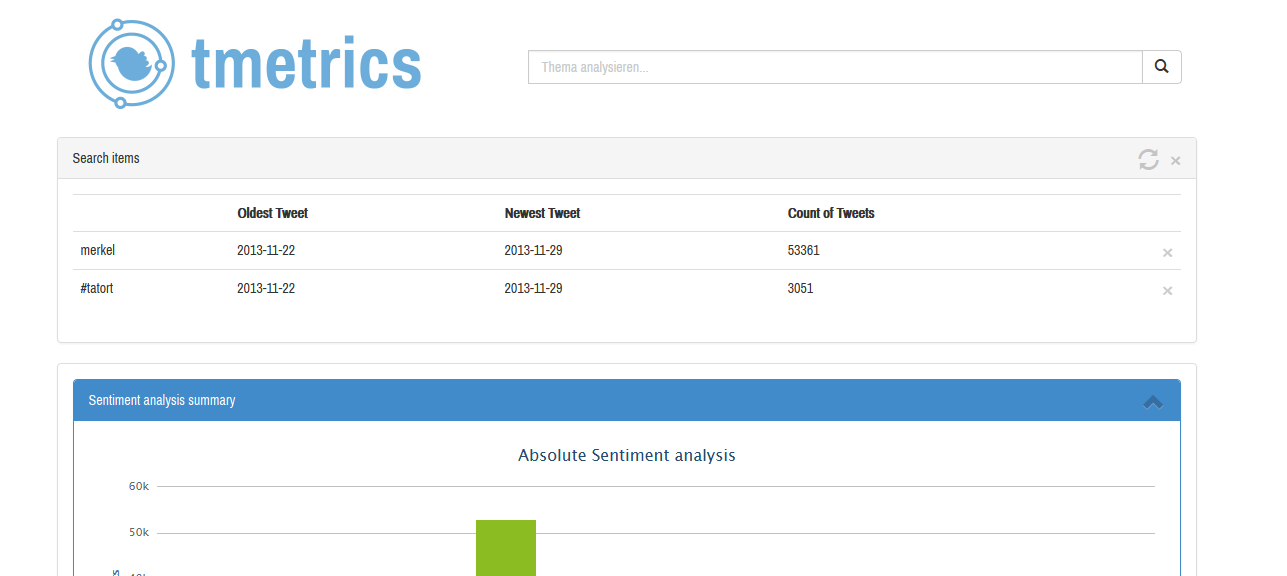
\includegraphics[width=0.8\textwidth]{./Bilder/Frontend/Screenshots/tabelleninterface.png}
\caption{Tabellarische Darstellung der Suchbegriffe}
\label{img:tabelle}
\end{figure}

Für die weiteren Ansichten wurde ein Konzept erarbeitet, welches diese Einfachheit und Übersichtlichkeit fortführen sollte. Grundsätzlich wurden das Logo und die Suchleiste verkleinert, weiter nach oben gerückt und nebeneinander anstatt untereinander angeordnet. Als dann die ersten Ergebnisse wie die Anzahl der gefundenen Tweets zu einem Suchbegriff, Datum der ersten und der neusten Suche zur Verfügung standen, wurden diese Daten tabellarisch dargestellt. Darunter wurden nach und nach untereinander die einzelnen Auswertungen hinzugefügt (siehe Abbildung \ref{img:tabelle}).

Nach der Eingabe eines weiteren neuen Begriffes öffnete sich zunächst immer die Vergleichsansicht. Dies entsprach grundsätzlich der Intention des gesamten Projektes, einzelne Begriffe miteinander vergleichen zu können. Um eine ausführlichere Auswertung zu einem einzelnen Begriff angezeigt zu bekommen, genügte ein Klick auf die jeweilige Tabellenzeile.

Im weiteren Verlauf des Projektes stellte sich doch heraus, dass dieses Bedienkonzept nicht besonders intuitiv zu sein schien. So musste für einen Wechsel zwischen der detaillierten Einzelansicht zweier verschiedener Begriffe mehrfach geklickt werden, was teilweise für den Benutzer nicht direkt nachvollziehbar war.

Außerdem stellte sich heraus, dass mit steigender Anzahl von Analyseansichten der Platz durch die Tabelle direkt im zentralen Fokus des Benutzers eher verschwendet wurde, anstatt diese Fläche mit einer höheren Informationsdichte z.B. in Form einer Analyse zu füllen. Nicht nur der Kunde, sondern auch die Entwickler merkten schnell, dass man hier viel scrollen musste, um die einzelnen Auswertungen dargestellt zu bekommen.

\subsubsection{Zweites Konzept: Kacheln}
\label{sec:konzeptKacheln}

\begin{figure}[h!]
 \centering
 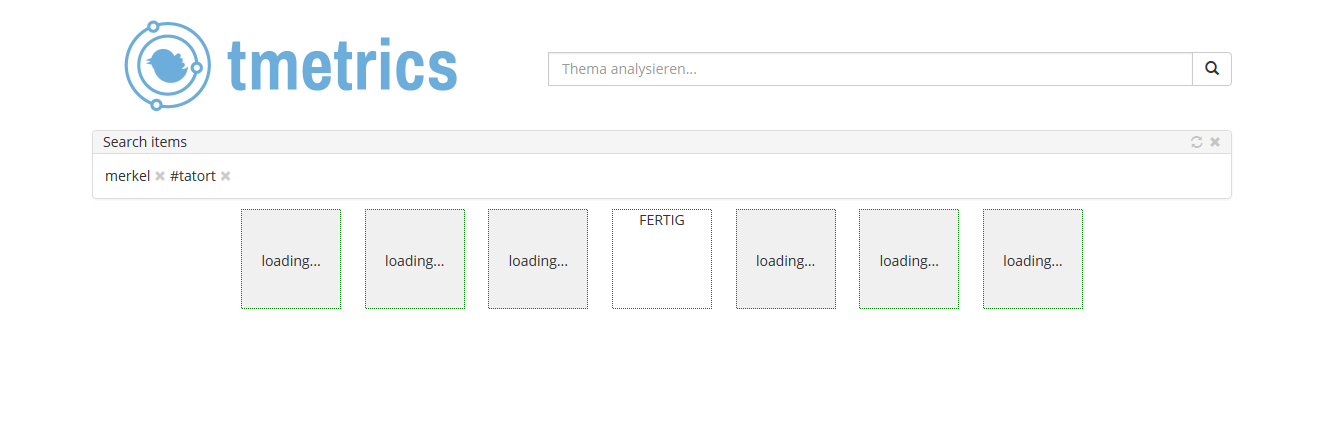
\includegraphics[width=0.8\textwidth]{./Bilder/Frontend/Screenshots/kachelinterface.png}
\caption{Erster Entwurf des Interfaces mit Kacheln, Arbeitsversion}
\label{img:kachel}
\end{figure}

In einem Sprint-Review schlug der Kunde also ein "`Kachelinterface"' vor. Der Hintergedanke des Kunden dabei war, dass ein "`exploratives"' Arbeiten ermöglicht werden sollte, indem man alle Auswertungen als mehr oder weniger große Kacheln direkt zu sehen bekommt und man durch ein Anklicken dieser Kachel in diese Analyseansicht "`hineingeht"', man sozusagen auch optisch und informativ in die Tiefe geht und dort dann die Details der jeweiligen Analyse angezeigt bekommt.

Während im Entwicklerteam die ersten Ideen und Ansätze (siehe Abbildung \ref{img:kachel}) zur Umsetzung heranreiften, stellte sich heraus, dass dies an vielen Stellen im Frontend einer völligen Neuentwicklung gleich käme, sich also nur mit erheblichem Aufwand umsetzen ließe. Außerdem fiel anhand erster Skizzen und Überlegungen zur optischen Gestaltung schnell auf, dass man hier für den eigentlich als essentiell erachteten Vergleich einer bestimmten Analyse zweier verschiedener Begriffe nur noch umständlich zugreifen kann. Grob umschrieben hätte sich der Interaktionsablauf so dargestellt, dass man eine geöffnete Analyse erst hätte schließen müssen, dann den Begriff wechseln um erneut im explorativen Stil wieder in die Tiefe gehen zu müssen.

Aus diesen Gründen beschäftigte sich das Team mit einem alternativen Ansatz. 

\subsubsection{Finales Konzept: Tabs}
\label{sec:konzeptTabs}
Erste Ideen zu diesem Konzept ergaben sich bereits während der Betrachtungen des Kachelinterfaces. Nachdem das Team diese Überlegungen weiter ausführte und gemeinsam mögliche Schwachstellen beseitigte wurde das neue Konzept dem Kunden in einem gesondertem Termin vorgestellt. Dieser war von der Idee begeistert und gab grünes Licht für die Umsetzung.
Das Konzept lehnt sich an das Kachelinterface des Kunden an, verbindet aber auch weitere bekannte strukturgebende Elemente wie z.B. verschiedene Tabs. Die Kacheln wurden aufgegriffen, um die Auswahl der zur Verfügung stehenden Analysemöglichkeiten darzustellen. Hier kann der Kunde die gerade aktiven und für alle Suchbegriffe gültigen Analysen einzeln aktivieren oder wieder deaktivieren. Diese Kachelansicht enthält exemplarische Darstellungen und kurze Beschreibungen der jeweiligen Analysen. Für einzelne Suchbegriffe werden nun Reiter anstelle von Tabelleneinträgen genutzt, diese können wie man es von modernen Browsern gewöhnt ist natürlich auch wieder geschlossen werden. Sobald mehr als ein Suchbegriff als Reiter geöffnet ist, erscheint als zusätzlicher Reiter ganz rechts der Comparison-Tab. Hier ist die Darstellung des direkten Vergleichs zweier Begriffe wiederzufinden. Aber auch der Vergleich anderer Analysen zu unterschiedlichen Begriffen ist mit diesem Konzept für den Benutzer deutlich einfacher zu realisieren. So kann er in der Analyseauswahl einfach nur die Analysen aktivieren, die für ihn gerade von Interesse sind. Um zwischen den Analysen der jeweiligen Begriffe hin- und herzuschalten, genügt jetzt ein einziger Klick auf den jeweiligen Tab.

Das ursprüngliche Ziel, ein simples und vor allem intuitives Interface zu gestalten, wurde durch die Verwendung von Reitern und weiteren bekannten optischen Elementen wie z.B. einem geöffnetem bzw. geschlossenem Auge zur Darstellung der aktiven bzw. inaktiven Analysen wieder erreicht.

\subsection{Verwendete Technologien}
Bereits vor und während der Phase eines ersten Entwurfs überlegten wir uns, welche externen Technologien und Bibliotheken uns bei der Entwicklung eines Frontends im Browser möglichst gut unterstützen könnten.

Dabei fiel schnell die Entscheidung, das HTML5-Framework Bootstrap \cite{Bootstrap} einzusetzen. Zwar muss man sich zusätzlich in dieses Framework einarbeiten und HTML5-Frameworks sind generell nicht mit älteren Browsern (wie beispielsweise Internet Explorer 8 oder älter) kompatibel, aber dafür bieten HTML5-Frameworks und im Speziellen Bootstrap auch zahlreiche Vorteile: Mit Hilfe vordefinierter Elemente (Icons, Buttons, Tabs, modale Dialoge, u.v.m.) sowohl in CSS als auch teilweise in JavaScript ist es möglich, ein homogenes Gesamtbild der Oberfläche zu erreichen, ohne selbst viele Anpassungen diesbezüglich machen zu müssen. Außerdem ist Bootstrap zu vielen aktuellen Browsern kompatibel, ohne dass der Entwickler einen Mehraufwand bzgl. der Kompatibilität betreiben muss \cite{BootstrapCompatibility}. Dies verdeutlicht Tabelle \ref{fig:BootstrapTab} anhand der Darstellung eines Buttons in verschiedenen Browsern mit und ohne Bootstrap.

Ebenfalls integriert ist der Ansatz von \textit{responsive webdesign}, das heißt, dass sich der Aufbau der Seite an das Endgerät des Benutzers anpassen kann, wofür im Allgemeinen CSS Media Queries \cite{CSSMediaQueries} eingesetzt werden. Beispielsweise ist es mit CSS Media Queries möglich, die Darstellung von HTML-Elementen an die Breite des Ausgabegerätes anzupassen. Speziell für Bootstrap spricht, dass der Quellcode frei verfügbar ist, viele Menschen es nutzen und somit auch viele Möglichkeiten für Hilfestellungen existieren, sowie die zahlreichen, verfügbaren Beispiele auf der Homepage, die gut dokumentiert sind.

\begin{table}[ht]
\centering
\small
\begin{tabular}{>{\raggedleft}c | m{2.25cm} | m{2.25cm} | m{2.25cm} | m{2.25cm}}
\toprule
 & Firefox & Chrome\newline(Windows) & IE 10 & Chrome\newline(Android)\\
\midrule
mit Bootstrap &

\includegraphics[width=2cm]{./Bilder/Frontend/Buttons/firefoxWith.png} &

\includegraphics[width=2cm]{./Bilder/Frontend/Buttons/chromeWith.png} &

\includegraphics[width=2cm]{./Bilder/Frontend/Buttons/ieWith.png} &

\includegraphics[width=2cm]{./Bilder/Frontend/Buttons/androidWith.png}
\\
\midrule
ohne Bootstrap &
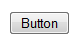
\includegraphics[width=2cm]{./Bilder/Frontend/Buttons/firefoxWithout.png} &
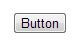
\includegraphics[width=2cm]{./Bilder/Frontend/Buttons/chromeWithout.png} &
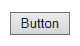
\includegraphics[width=2cm]{./Bilder/Frontend/Buttons/ieWithout.png} &
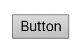
\includegraphics[width=2cm]{./Bilder/Frontend/Buttons/androidWithout.png}
\\
\bottomrule
\end{tabular} 
\caption{Vergleich der Darstellung eines Buttons in verschiedenen Browsern mit und ohne Bootstrap}
\label{fig:BootstrapTab}
\end{table}

Mit der Entscheidung für Bootstrap ging auch die Entscheidung für jQuery \cite{jQuery} als Werkzeug zur Navigation und Manipulation des Document Object Models, einem Interface zum dynamischen Zugriff auf die Struktur, den Inhalt und den Stil eines Dokuments, einher. Dies ist dadurch begründet, dass einerseits alle JavaScript-Elemente von Bootstrap jQuery benötigen und wir andererseits aus Erfahrung wussten, dass eine Bibliothek wie jQuery die Gestaltung einer Oberfläche mit Hilfe von JavaScript erheblich vereinfacht.

Zusätzlich zu diesen beiden Bibliotheken, die einen Rahmen zur Entwicklung der Oberfläche bieten, verwenden wir auch für die Darstellung der einzelnen Auswertungen zwei externe Bibliotheken.
Dies ist erstens Highcharts \cite{Highcharts}, welches die Darstellung verschiedener Graphen (beispielsweise Punktwolken, Balken- oder Kuchendiagramme) übernimmt. In der finalen Version unseres Systems wird Highcharts für die Darstellung von sieben der acht verfügbaren Auswertungen verwendet.
Für die Darstellung der achten Auswertung (namentlich die Ansicht \texttt{tagCloud}) verwenden wir die D3 Word Cloud \cite{D3TagCloud}, welche Anordnung, Sklaierung und Färbung der Wörter in der Tag Cloud berechnet und anschließend darstellt.

\subsection{Datenhaltung}
Bereits während der ersten Iteration unseres Projekts ergab sich das Bedürfnis, Antworten des REST-Services zwischenzuspeichern, solange sich der Benutzer auf TMetrics befindet, um möglichst selten neue Anfragen an den REST-Service senden zu müssen. Dies wurde vor allem dann deutlich, wenn bereits mindestens zwei Suchbegriffe eingegeben waren und man zwischen diesen hin- und herwechselte. Bei jedem Wechsel wurden die Anfragen für alle Auswertungen zum Suchbegriff, auf den man wechselte, neu abgeschickt.
Die erste Idee, diesem Problem zu entgegnen, war eine Zwischenspeicherung der Daten im Frontend. Da es sich bei den Antworten des REST-Services wie in Abschnitt \ref{sec:architekturDarstellung}
erwähnt um JSON-Objekte handelt, war eine Speicherung dieser ohne großen Zusatzaufwand möglich. Die Frage war nun, wo diese JSON-Objekte abgespeichert werden sollten. Da jedes JSON-Objekt immer genau einem Suchbegriff und einem Suchbegriff mehrere JSON-Objekte (für jede Auswertung ein Objekt) zugeordnet waren, war die erste Idee die in \texttt{jQuery} enthaltene Funktion \texttt{data(key, value)} zu nutzen. Diese Funktion speichert zu einem oder mehreren HTML-Elementen ein beliebiges JavaScript-Objekt \texttt{value} unter dem Schlüssel \texttt{key} ab. Das abgespeicherte Objekt kann mit der Funktion \texttt{data(key)} und demselben Schlüssel dann wieder abgerufen werden \cite{jQueryData}.

Da in der ersten Version des Frontends zu jedem Suchbegriff auch eine Zeile in der in Abschnitt \ref{sec:konzeptTabelle} beschriebenen Tabelle, also ein \texttt{<tr>}-Element, existierte, war die Idee jeder Anfrage einen eindeutigen Schlüsselnamen zu geben und so das entsprechende JSON-Objekt mit diesem Schlüsselnamen an der zu diesem Suchbegriff passenden Tabellenzeile zu speichern. Beim Abrufen einer Auswertung wurde dann, falls verfügbar, auf das zwischengespeicherte JSON-Objekt zugegriffen und ansonsten eine neue Anfrage an den REST-Service gestellt.

Allerdings war diese Umsetzung der Datenhaltung an die Darstellung als Tabelle gebunden, was bei der Umstellung auf ein neues Darstellungskonzept, wie in \ref{sec:konzeptKacheln} beschrieben, zu Problemen führte. Es wäre möglich gewesen, die Daten nun an den neuen HTML-Objekten zu speichern, was das Problem allerdings nur temporär bis zur eventuell nächsten Umstellung des Designs gelöst hätte.
Für eine langfristige Lösung war es also von Nöten, Datenhaltung und Darstellung unabhängig voneinander zu gestalten.

\begin{figure}
 \centering
 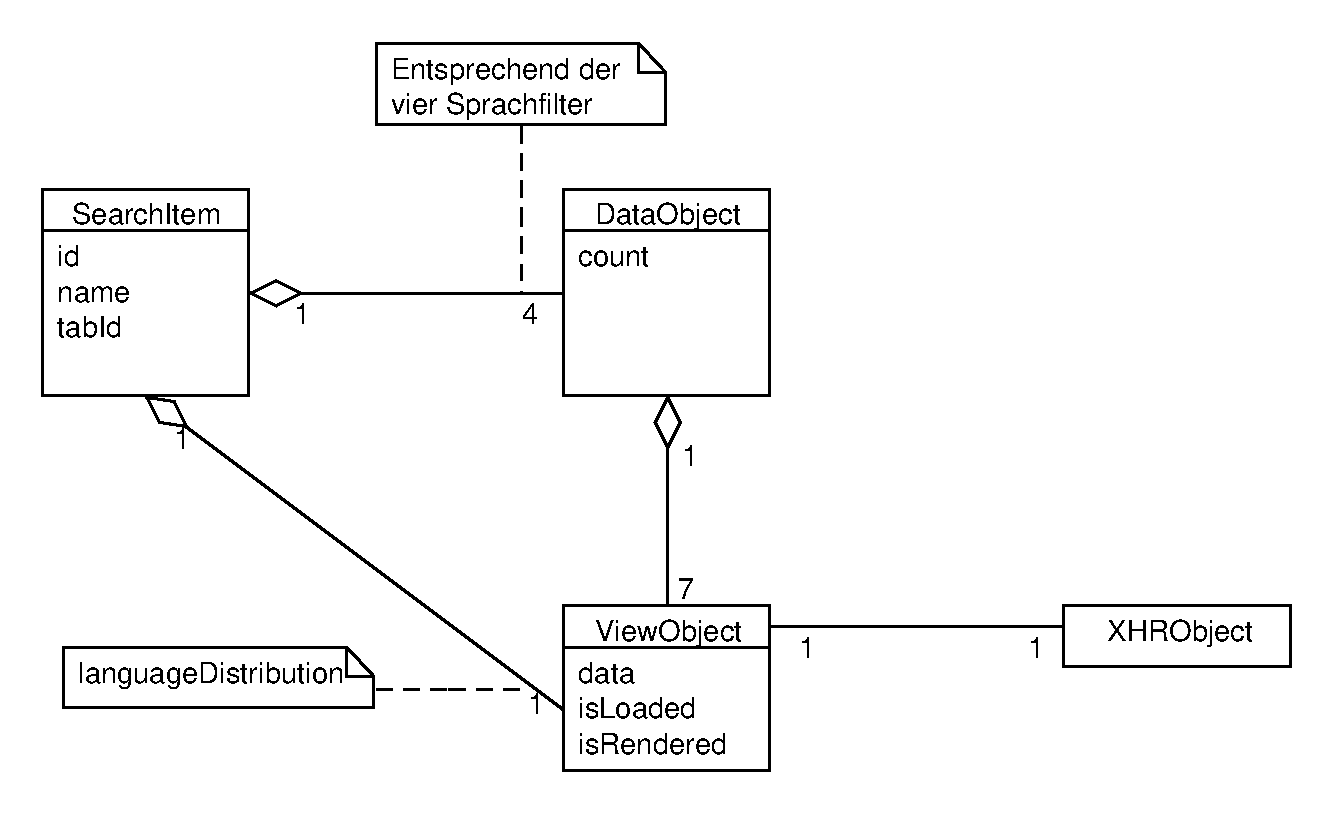
\includegraphics[width=0.8\textwidth]{./Bilder/Frontend/classDiagram.pdf}
\caption{Klassendiagramm der Datenhaltung im Frontend}
\label{img:FrontEndClassDiagram}
\end{figure} 

Die Umsetzung dieser Idee ist in der in Abbildung
\ref{img:FrontEndClassDiagram}
dargestellten Klassenstruktur eines globalen Arrays von Suchbegriffen gemündet. Dabei wird für jeden Suchbegriff (Klasse \texttt{SearchItem}) zwischen vier vordefinierten Sprachfiltern (keine Filterung, englisch, deutsch und eine beliebige weitere Sprache; Klasse \texttt{DataObject}) und in jedem Filter nochmals zwischen den acht verfügbaren Ansichten (Klasse \texttt{ViewObject}) unterschieden. Die einzige Ausnahme hiervon bildet die Ansicht \texttt{languageDistribution}, weil diese unabhängig vom eingestellten Sprachfilter ist und daher nur einmal pro Suchbegriff gespeichert werden muss.
Als zusätzliche Information wird zu jedem \texttt{DataObject} abgespeichert, wie viele Tweets zu diesem Suchbegriff mit dem jeweiligen Sprachfilter vorliegen.
Zu jeder einzelnen Ansicht wird wiederum einerseits, falls vorhanden, das JSON-Objekt der Antwort einer Anfrage des REST-Services zusammen mit den Informationen, ob die Ansicht fertig geladen und gerendert wurde (jeweils als \texttt{boolean}-Flag), gespeichert. Andererseits wird die REST-Anfrage selbst als eigenes Objekt \texttt{XHRObject} für die Verwendung in den \textit{connection pools} gespeichert, die im nächsten Abschnitt \ref{sec:conPool} beschrieben werden.
Außerdem sind noch der aktive Tab, der aktive Sprachfilter und ein \texttt{boolean}-Array, das angibt, welche Ansichten sichtbar bzw. nicht sichtbar sind, global verfügbar, sodass jederzeit bekannt ist, welche Ansichten der Benutzer aktuell angezeigt bekommt und welche Daten dafür benötigt werden.

Zusätzlich zu der gerade beschriebenen flüchtigen Speicherung von Daten im Frontend, wird auch eine persistente Speicherung für benutzerspezifische Einstellungen verwendet. Dabei werden die Einstellungen zur Sichtbarkeit der Ansichten und der gewählte Sprachfilter über den \texttt{localStorage} \cite{WebStorage} client-seitig gespeichert. Zudem werden auch die aktuellen Suchbegriffe gespeichert, sodass diese beim nächsten Besuch von TMetrics dem Benutzer in einem Dropdown-Menü zur erneuten Analyse vorgeschlagen werden. Hierbei werden aber immer nur die Suchbegriffe des direkten vorherigen Besuchs gespeichert.

\subsection{Connection Pools}
\label{sec:conPool}
\subsubsection{Problematik}
Bedingt durch die REST-Architektur unseres Systems und die Entscheidung, einzelne Ansichten unabh"angig voneinander aufrufen zu k"onnen, wird in unserem System f"ur jede Ansicht (einen Überblick über die Ansichten von TMetrics wurden in Abschnitt \ref{sec:umgesetztesSystem} gegeben und sind in Abbildung \ref{fig:viewScreenshots} zu sehen) eine Anfrage an den REST-Service gestellt. 
Alle g"angigen Browser unterst"utzen aber nur eine gewisse Anzahl an parallelen Verbindungen pro Server (siehe Tabelle \ref{fig:ConPoolTab}). Das Minimum der Anzahl paralleler Verbindungen zu einem Server unter den von uns unterst"utzen Browsern liegt bei sechs. 

\begin{table}[ht]
\centering
\small
\begin{tabular}{l | c c c c c c c}
\toprule
Browser & Parallele Verbindungen\\
\midrule
Chrome 4+ & 6\\
Firefox 3+ & 6\\
IE 8 \& 9 & 6\\
IE 10 & 8\\
Opera 10 & 8\\
Opera 11+ & 6\\
Safari 4+ & 6\\ 
\bottomrule
\end{tabular} 
\caption{Anzahl paralleler Verbindungen zu einem Server verschiedener Browser und Versionen \cite{BrowserScope}.}
\label{fig:ConPoolTab}
\end{table}

Gibt der Benutzer im Frontend einen Suchbegriff ein und schickt diesen ab, so werden f"ur die Ansichten bereits acht Anfragen an den REST-Service geschickt, was  acht parallelen Verbindungen zu einem Server entspricht. Der Browser des Benutzers wird in diesem Fall aber zun"achst nur so viele Anfragen abschicken, wie seine Konfiguration es zulässt. Wie oben beschrieben gehen wir hierbei im schlechtesten Fall von sechs Anfragen aus. Die verbleibenden anderen beiden Anfragen werden solange zur"uckgehalten, bis auf eine der vorherigen eine Antwort des REST-Services kommt.

Dies ist soweit noch kein Problem, da der Benutzer lediglich f"ur zwei Auswertungen l"anger warten muss, als diese Auswertungen eigentlich an Zeit ben"otigen. Problematisch wird es, wenn der Benutzer direkt nach Eingeben des ersten Suchbegriffs einen weiteren Suchbegriff eingibt, da auch dabei schon bevor die acht Anfragen der Auswertungen abgeschickt werden, bis zu zwei weitere sequentielle Anfragen an den REST-Service geschickt werden. Zuerst die Anfrage, ob der Suchbegriff bereits in der Datenbank vorliegt und falls dies zutrifft die Anfrage, die die interne ID dieses Suchbegriffs zur"uckliefert. Erst nach der Antwort auf diese beiden initialen Anfragen wird dem Benutzer ein Feedback im Frontend in Form des Erscheinen eines neuen Tabs für den soeben abgeschickten Suchbegriff gegeben und die Anfragen der einzelnen Ansichten werden abgeschickt.

Im ung"unstigen Fall, dass nun alle sechs Verbindungen zum Server durch Anfragen der Ansichten belegt sind, wird beim Abschicken eines neuen Suchbegriffs die Anfrage, ob dieser Begriff bereits in der Datenbank vorliegt, zun"achst nicht abgeschickt und der Benutzer bekommt somit auch kein Feedback vom Frontend.

Zur L"osung dieser Problematik haben wir zwei Ans"atze in Betracht gezogen. Erstens das Zusammenf"uhren von Anfragen, sodass wir insgesamt deutlich weniger Verbindungen pro Server ben"otigen und zweitens die Einf"uhrung eines Verwaltungssystems f"ur Anfragen, sodass wir an Stelle des Browsers regeln, welche Anfragen gestartet und welche noch warten sollen.
Das f"ur unsere Entscheidung ausschlaggebende Argument war, dass f"ur den Benutzer h"aufig nicht alle Ansichten relevant sind. Das hei\ss{}t, dass er in den Einstellungen zur Sichtbarkeit die Ansichten ausgew"ahlt hat, die er angezeigt bekommen m"ochte. Unser System sollte also die Anfragen zu diesen Ansichten bevorzugt behandeln. Dies w"are mit dem ersten L"osungsvorschlag nicht m"oglich, da alle Anfragen zu einer geb"undelt w"urden und eine Antwort auf diese geb"undelte Anfrage erst k"ame, wenn alle Teilauswertungen vom REST-Service bearbeitet w"aren.
Der Benutzer m"usste also im schlimmsten Fall auf die Auswertung einer Ansicht warten, die er nicht sehen m"ochte.
Unser L"osungsansatz ist also die Einf"uhrung eines Verwaltungssystems f"ur Anfragen, welches wir \textit{connection pools} nennen.

\subsubsection{Aufbau}
Die Idee der \textit{connection pools} ist es, Anfragen nach Priorit"aten zu behandeln und abzuarbeiten. Dabei gibt es folgende drei Priorit"aten: passiv, aktiv und spezial. F"ur jede existiert jeweils ein Pool mit momentan in Bearbeitung stehenden Anfragen und eine Warteschlange f"ur noch zu bearbeitende Anfragen. Die Aufgabe der \textit{connection pools} ist es nun, daf"ur zu sorgen, dass einerseits in den Pools der drei Priorit"aten zusammen maximal sechs Verbindungen zum Server existieren und andererseits die Pools mit Anfragen aus den Warteschlangen aufgef"ullt werden, wenn eine Anfrage abgearbeitet wurde.

\subsubsection{Umsetzung}
Zur Realisierung dieser Aufgaben wird jedem der drei Pools eine feste Anzahl an erlaubten Verbindungen zum Server, sogenannte Slots, zugeteilt. In unserem System stehen f"ur den Spezial-Pool ein, f"ur den Aktiv-Pool drei und f"ur den Passiv-Pool zwei Slots zur Verf"ugung. Diese Zuteilung ergab sich aus der Überlegung, welche Anfrage mit einer bestimmten Priorit"at in welcher H"aufigkeit auftritt.

Da nur die Anfragen nach der ID eines Suchbegriffs und ob ein Suchbegriff bereits in der Datenbank vorliegt, die Priorit"at spezial haben und diese Anfragen nie parallel ausgef"uhrt werden, gen"ugt logischerweise ein Slot f"ur den Spezial-Pool. Diese Anfragen sollten also schnellstmöglich abgeschickt werden, um das eingangs genannte Problem zu lösen. Alle anderen Anfragen haben entweder die Priorit"at aktiv, wenn der Benutzer die Ergebnisse der Anfrage direkt angezeigt bekommen soll oder passiv, falls die Anfrage nur im Hintergrund l"auft und Ergebnisse dann auf Abruf bereit stehen sollen. Dies ist abh"angig vom aktiven Tab, dem ausgew"ahlten Sprachfilter, sowie der Einstellung f"ur die Sichtbarkeit der einzelnen Ansichten.
Eine andere Verteilung der Slots von Passiv- und Aktiv-Pool ist auch m"oglich und einfach im Code anzupassen.

Bei den Warteschlangen handelt es sich um Stacks bzw. LIFO-Warteschlangen. Dies hat den Hintergrund dass wir dem Benutzer generell das Ergebnis, auf die von ihm zuletzt ausgef"uhrte Aktion am schnellsten liefern möchten, damit die aktuelle Anzeige im Frontend mit Daten gefüllt ist.

Ein weitere Idee der Umsetzung der \textit{connection pools} ist es, dass auf Eingaben des Benutzers angemessen reagiert wird. Das bedeutet, dass die Priorit"aten von Anfragen ge"andert werden, wenn sich die Sichtbarkeit der zugeh"origen Ansichten als Folge einer Nutzereingabe "andert. Dies kann durch Wechsel des Tabs, des Sprachfilters oder der Sichtbarkeitseinstellung geschehen. Eine Anfrage zu einer Ansicht, die nicht mehr sichtbar ist, wird, sofern sie noch nicht fertig abgearbeitet ist, abgebrochen und in den Passiv-Pool bzw. in die Passiv-Warteschlange verschoben. Im umgekehrten Fall wird in den Aktiv-Pool bzw. in die Aktiv-Warteschlange verschoben.
So wird sichergestellt, dass die Priorit"aten aller Anfragen zu jeder Zeit an die Aktionen des Nutzers angepasst sind und Anfragen relevanter Ansichten m"oglichst schnell bearbeitet werden.

\subsubsection{Fazit}
Ein Problem der \textit{connection pools} ist es, dass damit nur Anfragen verwaltet werden, die wir auch aktiv zuweisen. Dies ist bei Anfragen, die "uber externe Bibliotheken abgeschickt werden, nicht ohne Weiteres m"oglich. Dies betrifft in unserem System die Autovervollst"andigung bei Eingabe eines Suchbegriffs. In diesem Fall wird in der Bibliothek \texttt{typeahead.js} \cite{typeahead}
geregelt, wann genau eine Anfrage abgeschickt wird und wir k"onnen sie daher nicht in die \textit{connection pools} einpflegen. Um dieses Problem zu l"osen, w"are eine Anpassung der externen Bibliothek n"otig.

Ein weiteres mit den \textit{connection pools} verbundenes Problem ist die teilweise schlechte Auslastung der einzelnen Pools. Da eine Anfrage eine festgelegte Priorit"at hat, ist sie auch fest einem Pool, bzw. einer Warteschlange zugeordnet. Will der Benutzer aber beispielsweise die Auswertungen zu allen Ansichten haben, so werden acht Anfragen an die Connection Pools gesendet, von denen aber nur drei direkt abgeschickt werden, da der Aktiv-Pool nur drei Slots hat. Ohne die \textit{connection pools} w"aren an dieser Stelle sechs Anfragen abgeschickt worden. Eine m"ogliche L"osung w"are die Nutzung von Pools anderer Priorit"aten unter der Bedingung, dass diese entweder frei sind oder eine niedrigere Priorit"at haben. So w"urden Anfragen der Priorit"at aktiv nur den Spezial-Pool benutzen, wenn dieser frei w"are (und von m"oglicherweise ankommenden Anfragen mit Priorit"at spezial wieder verdr"angt werden). Der Passiv-Pool hingegen k"onnte direkt von Anfragen mit Priorit"at aktiv genutzt werden. Mögliche Anfragen der Priorität passiv sollten dabei von denen der Priorität aktiv verdrängt werden.

Zusammenfassend lässt sich sagen, dass die \textit{connection pools} eine funktionierende Umsetzung f"ur eine Verwaltung von Anfragen an den Server sind. Um die Effizienz voll auszureizen, sollten aber die in diesem Unterabschnitt genannten Probleme noch behoben werden.

\subsection{Besonderheiten}

In diesem Abschnitt werden weitere interessante Details der Implementierung oder Designentscheidungen, die wir bezüglich des Frontends getroffen haben, diskutiert.

\subsubsection{Anzahl an Tweets im zeitlichen Verlauf}

Die im Folgenden beschriebene Ansicht gibt an, wie viele Tweets zu einem gegebenen Suchbegriff in einem bestimmten Zeitraum veröffentlicht wurden.

Bei der ersten Implementierung dieser Ansicht haben wir festgelegt, dass die Tweets eines Tages jeweils addiert werden, sodass der Graph die Anzahl Tweets pro Tag widerspiegelte.
Wie in Abbildung \ref{fig:tphCompare} deutlich wird, wird die Auswertung vor allem bei Suchbegriffen, zu denen nur über einen verhältnismäßig kurzen Zeitraum Daten vorliegen, aussagekräftiger, wenn man den betrachteten Zeitraum von einem Tag auf eine Stunde verkürzt.

Aber auch hierbei ist eine weitere Optimierung denkbar, da die Anzahl Tweets pro Stunde an Aussagekraft verlieren, wenn man einen Datenbestand betrachtet, der sich über einen großen Zeitraum, beispielsweise mehrere Monate, erstreckt. Eine Anpassung des zusammenzufassenden Zeitraums in Abhängigkeit vom gesamten betrachteten Zeitraum wäre also wünschenswert, um diese Problematik zu lösen. Eine leichte Umsetzung dieser Idee ist allerdings nicht möglich, da Highcharts diese Funktionalität nicht nativ unterstützt und man dies manuell einbauen müsste.
Im Verlauf des Projektes wurde allerdings weitere Funktionalität in die hier beschriebene Ansicht eingefügt. Nachdem der Kundenwunsch nach explorativem Arbeiten in unserem System laut wurde, wurde einerseits das durch Klick auf den Graphen aufrufbare Anzeigen von einzelnen Tweets einer bestimmten Stunde (siehe Abschnitt \ref{sec:showTweets}) implementiert. Andererseits wurde dann auch noch das in Abschnitt \ref{sec:news} beschriebene News-Modul in diese Ansicht integriert. Details dazu sind den jeweiligen Abschnitten zu entnehmen.

\begin{figure}[ht]
\centering
\begin{subfigure}[t]{0.45\textwidth}
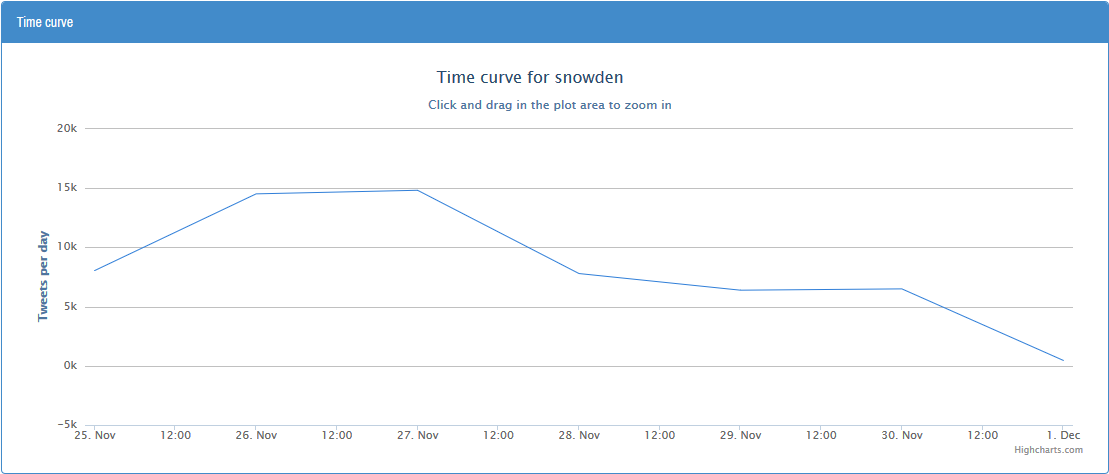
\includegraphics[width=\textwidth]{Bilder/Frontend/snowdenOld.png}
\caption{Tweets pro Tag}
\label{fig:tphDay}
\end{subfigure}
~
\begin{subfigure}[t]{0.45\textwidth}
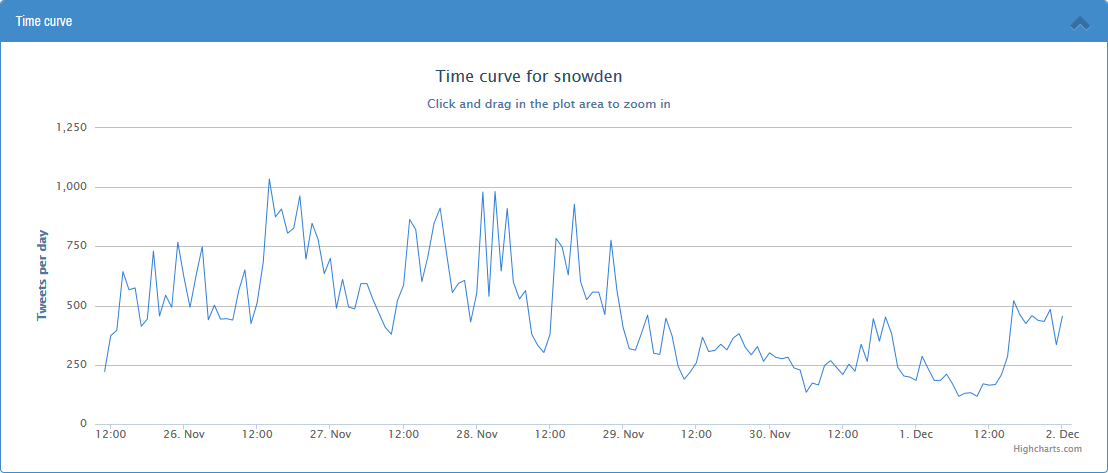
\includegraphics[width=\textwidth]{Bilder/Frontend/snowdenNew.png}
\caption{Tweets pro Stunde}
\label{fig:tphHour}
\end{subfigure}
\caption{Vergleich der Tweets im zeitlichen Verlauf pro Tag (links) und pro Stunde (rechts) zum Suchbegriff \glqq Snowden\grqq}
\label{fig:tphCompare}
\end{figure}

\subsubsection{Tweets anzeigen}
\label{sec:showTweets}
Wie bereits im vorigen Abschnitt erwähnt, bietet TMetrics die Möglichkeit, explorativ zu arbeiten und sich einzelne Tweets anzeigen zu lassen. Diese Funktionalität ist einerseits in der Auswertung der Sentiment-Analyse verfügbar und andererseits in der Ansicht der Anzahl Tweets im zeitlichen Verlauf. Aus der Sentiment-Analyse heraus werden je nachdem, welcher Teil des Balken- oder Kuchendiagramms angeklickt wurde, nur positive, nur negative oder nur neutrale Tweets angezeigt. Will man einzelne Tweets aus der Ansicht des zeitlichen Verlaufs heraus betrachten, so werden nur Tweets innerhalb des ausgewählten Zeitraums, also innerhalb einer bestimmten Stunde, angezeigt.

Unabhängig von der Ansicht, ist die Anzeige einzelner Tweets auf maximal 100 Tweets begrenzt. Eine solche Begrenzung ist sinnvoll, da sonst bei einem Suchbegriff mit großem Datenbestand sehr lange Ladezeiten verursacht werden können.
Um dem Nutzer nun dennoch möglichst repräsentative Tweets zeigen zu können, werden die Tweets nach Wichtigkeit sortiert. Als Maß für die Wichtigkeit eines Tweets sind verschiedene Möglichkeiten denkbar. Wir haben uns dafür entschieden, die Anzahl Retweets eines Tweets als alleiniges Maß für die Wichtigkeit eines Tweets zu nehmen. Grund für diese Entscheidung ist, dass die Anzahl Retweets ein eigenes Feld der Datenbank ist und wir daher effizient sortieren können, um die 100 wichtigsten Tweets zu finden. Da aber auch einem Retweet selbst dieselbe Anzahl an Retweets wie dem Original-Tweet zugeordnet ist, hat dies zur Folge, dass wir Retweets von der Anzeige ausschließen müssen, um eine mehrfache Anzeige des gleichen Tweets zu vermeiden. Es werden also die 100 Original-Tweets mit der höchsten Anzahl an Retweets angezeigt.

Ein weiteres Feature der Anzeige einzelner Tweets ist die Anzeige von weiteren Informationen zu diesem Tweet, die auf Wunsch abrufbar sind. So ist es durch einen einfachen Klick auf den Namen des Autors eines Tweets möglich, nähere Informationen über diesen einblenden zu lassen. Selbiges gilt auch für einen Klick auf den Text des Tweets, was eine Anzeige der Anzahl Retweets, der geografischen Koordinaten (falls verfügbar), der Sprache, sowie des Sentiments des Tweets zur Folge hat. Hier wird dem Benutzer wiederum die Möglichkeit gegeben, sich näher über die Einflussfaktoren des Sentiments zu informieren, was im folgenden Abschnitt \ref{sec:showTweetsSenti} näher erläutert wird. Bei der Designentscheidung war es besonders wichtig, den Fokus zunächst auf das Wesentliche -- also den Tweet selbst -- zu legen und trotzdem die Möglichkeit zu bieten, detaillierte Informationen dem Nutzer auf Abruf zur Verfügung zu stellen.

\subsubsection{Darstellung der Sentiment-Einflussfaktoren}
\label{sec:showTweetsSenti}
Aus dem Anspruch, dem Benutzer ein exploratives Arbeiten auf TMetrics zu ermöglichen, ergab sich im Projektverlauf die Anforderung, eine Möglichkeit zu liefern, die Einflussfaktoren bei der Bestimmung des Sentiments eines Tweets darzustellen. Grundsätzlich existieren dabei zwei Kategorien von Einflussfaktoren auf das Sentiment eines Tweets: ein vorbestimmtes Wörterbuch (für Wörter und Emoticons) mit festgelegten Sentiment-Werten sowie ein auf Trainingsdaten basierendes Regressionsmodell mit Werten für sämtliche Wörter (Unigrams) sowie Wortgruppen aus zwei bis vier Wörtern (Bigrams, Trigrams und Fourgrams, siehe auch Abschnitt \ref{sec:regressionmodel}).  Daraus ergeben sich insgesamt sechs Faktoren, deren Summe das Sentiment des Tweets bestimmt: Wörter, Emoticons, Unigrams, Bigrams, Trigrams und Fourgrams.

Da für jeden Faktor auch noch angegeben werden soll, wie die Wörter im Tweet den Einfluss dieses Faktors beeinflussen, muss eine Menge Informationen wiedergegeben werden. Zur gleichen Zeit sollte die Größe der Box zum Anzeigen eines Tweets möglichst gering sowie die Darstellung der und Navigation zwischen den Einflussfaktoren möglichst intuitiv gehalten werden. Die Umsetzung dieser Anforderungen ist im Anschluss beschrieben.

\begin{figure}[ht]
\centering
\begin{subfigure}[t]{0.45\textwidth}
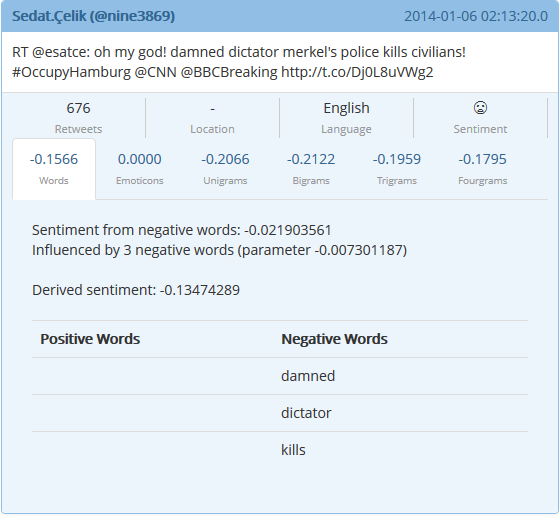
\includegraphics[width=\textwidth]{Bilder/Frontend/SentimentTweetsWords.png}
\caption{Wörterbuch}
\label{sentimenttweetswords}
\end{subfigure}
~
\begin{subfigure}[t]{0.45\textwidth}
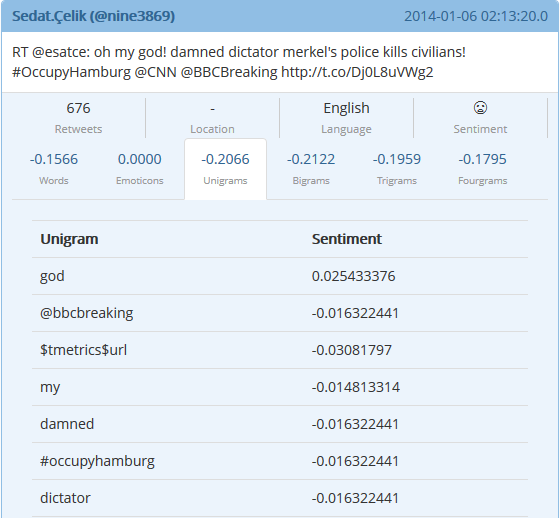
\includegraphics[width=\textwidth]{Bilder/Frontend/SentimentTweetsUnigrams.png}
\caption{n-Gramm}
\label{sentimenttweetsunigrams}
\end{subfigure}
\caption{Darstellung der Einflussfaktoren des Sentiments}
\label{sentimenttweets}
\end{figure}

Es wurde eine zusätzliche Ansicht hinzugefügt, die ausgehend von der Leiste mit den Metadaten durch Klick auf die Sentiment-Sparte ausgeklappt werden kann. Diese besteht dann aus sechs Tabs, welche den sechs genannten Einflussfaktoren entsprechen. Der Name des Reiters beinhaltet den Wert des Einflussfaktors, sodass die Summe der Werte aller Reiter dem Gesamtsentiment entspricht. Ein Klick auf den Reiter stellt eine detaillierte Auflistung dar, wie sein Wert aus dem Text des Tweets zustande kommt. Diese unterscheidet sich für die zwei eingangs genannten Kategorien.

Für Wörterbuch-Faktoren (in Abbildung \ref{sentimenttweetswords} exemplarisch für Wörter) basiert der Wert nur auf der Anzahl gefundener negativer bzw. positiver Wörter/Emoticons und einem zugehörigen Parameter. Ist mindestens ein solches Wort vorhanden, werden diese Werte und daraus berechnete (positive oder negative) Teil-Sentiment dargestellt. Der dabei dargestellte abgeleitete Sentiment-Wert ("`derived sentiment"') entspricht der Aggregationsfunktion zum Wörterbuch von Liu (siehe Abschnitt \ref{sec:sentimentclassifier}). Dieser wird immer angezeigt. Abschließend werden sämtliche im Wörterbuch vorkommenden Wörter des Tweets gelistet.

Die Darstellung der Details von Unigrams (für Unigrams in Abbildung \ref{sentimenttweetsunigrams} analog für Bigrams, Trigrams, Fourgrams) besteht nur aus einer tabellarischen Auflistung dieser n-Gramms des Tweets und der dazugehörigen Sentimentwerte (der Gesamtwert des Einflussfaktors entspricht der Summe seiner n-Gramms).

Zur besseren visuellen Aufbereitung dieser Informationen wird außerdem noch eine Einfärbung der n-Grams nach ihrem Sentiment-Wert vorgenommen. Dabei wurde die Konvention verwendet, neutrales Sentiment wie gewöhnlich in Schwarz darzustellen, während positives und negatives Sentiment in vier grünen bzw. roten Farbtönen mit zunehmender Sättigung dargestellt wird. Die dabei notwendige Festlegung wurde nach Betrachtung des Wertebereichs des Sentiments einzelner n-Grams intuitiv vorgenommen. Für positive n-Grams wurde festgestellt, dass nur sehr positive n-Grams den Wert 0.05 überschreiten, weshalb dies als untere Grenze für den grünen Farbton mit der höchsten Sättigung verwendet wurde. Weiterhin haben wir es als sinnvoll erachtet, dass nur dann ein positives Sentiment vorliegt, wenn die zweite Nachkommastelle nicht null ist. Daher wurde 0.1 als obere Grenze des neutralen Sentiments und damit als Untergrenze des grünen Farbtons mit der niedrigsten Sättigung verwendet. Danach fiel die Wahl auf 0.25 und 0.4 als Grenzwerte zwischen den übrigen Farbtönen. Da das Sentiment vom Modell her symmetrisch ist, wurden dieselben Grenzen im Negativen für die roten Farbtöne des negativen Sentiments verwendet. Da im Wörterbuch alle positiven Einträge gleich positiv und alle negativen Einträge gleich negativ sind, haben wir dort von einer Einfärbung abgesehen, da sie keine weiteren Informationen liefert.

Nachdem auf diese Weise bereits eine Heuristik zur Einfärbung von n-Grams implementiert worden ist, wurde die Entscheidung getroffen, sie auch auf den Gesamttext des Tweets anzuwenden. Eine Einfärbung auf Grundlage sämtlicher n-Grams ist dabei nicht praktikabel, da nicht für alle Wörter im Text ein eindeutiges Sentiment existiert. Es könnte z.B. ein Bigram mit negativem Sentiment existieren, das ein Unigram mit positivem Sentiment beinhaltet. Außerdem ist das Einfärben nur im Fall der Unigrams trivial, da sich dort der Text leicht in seine Wortbestandteile zerlegen lässt und sich diese anhand des Sentimentwertes des entsprechenden Unigrams einfärben lassen. Aus diesem Grund wurde das Einfärben nur für Unigrams umgesetzt. Die ursprüngliche Zielsetzung, die Einfärbung vom offenen Tab in der Ansicht der Einflussfaktoren abhängig zu machen und bei geschlossener Detailansicht gar keine Einfärbung im Volltext vorzunehmen, konnte aus Zeitgründen nicht umgesetzt werden, ist aber grundsätzlich möglich und sinnvoll. Unter diesen Umständen wäre es außerdem auch möglich, eine Einfärbung des Volltexts auf Grundlage des Wörterbuchs vorzunehmen. Beide Arten der Einfärbung sind in Abbildung \ref{sentimenttweetscolors} zu sehen.

\begin{figure}[ht]
\centering
\begin{subfigure}[t]{0.45\textwidth}
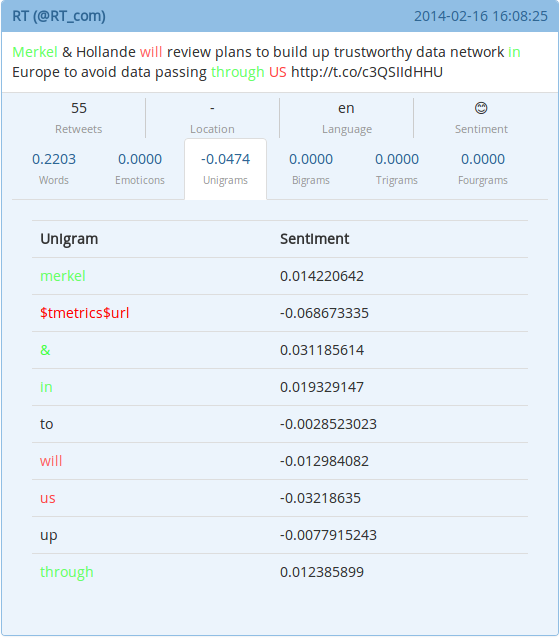
\includegraphics[width=\textwidth]{Bilder/Frontend/SentimentTweetsColors.png}
\caption{Einfärbung: n-Grams und Volltext}
\label{sentimenttweetscolors}
\end{subfigure}
~
\begin{subfigure}[t]{0.45\textwidth}
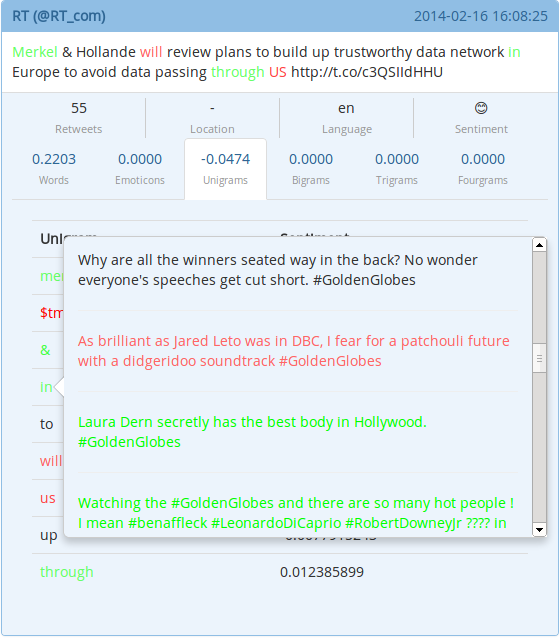
\includegraphics[width=\textwidth]{Bilder/Frontend/SentimentTrainingstweets.png}
\caption{Trainingstweets als Popover}
\label{trainingstweets}
\end{subfigure}
\caption{}
\end{figure}

Bei Betrachtung der Einflussfaktoren ist es möglich, dass die Fragestellung auftritt, wie das Sentiment dieses Faktors zustande gekommen ist (beispielsweise bei einem negativen Wert für ein intuitiv positives Wort). Aus diesem Grunde kann es von Interesse sein, sich die Trainingstweets anzuschauen, die zu dieser Bewertung des Sentiments geführt haben. Da unter Umständen viele Trainingstweets zu einem n-Gram vorliegen und jedes Mal deren Volltext dargestellt werden muss, stellt sich wieder die Herausforderung, diese Menge an zusätzlichen Informationen intuitiv und ohne Verkomplizierung des bestehenden Interfaces darzustellen. Dies wurde schlussendlich durch die Möglichkeit gewährleistet, auf ein n-Gram zu klicken und damit ein scrollbares Popover zu öffnen, welches nur den Text der relevanten Trainingstweets auflistet. Da Trainingstweets nur mit den Werten -1, -0.5, 0, 0.5 und 1 gelabelt werden können, ist es außerdem nicht notwendig, diese Werte explizit aufzulisten. Stattdessen wird das Labeling der Trainingstweets durch entsprechendes Einfärben des gesamten Textes in entsprechenden Farbtönen analog zur Einfärbung der n-Grams dargestellt. Ein Beispiel für die Darstellung der Trainingstweets kann man in Abbildung \ref{trainingstweets} sehen.

\subsubsection{Sentiment im zeitlichen Verlauf}
Schon sehr früh im Verlaufe des Projektes war es möglich, den Verlauf des Meinungsbildes zu einem konkreten Suchbegriff darzustellen. Hierzu wurde der anteilige Verlauf der positiven und der negativen Tweets mittels zweier sich überlagernder Kurven dargestellt. (Siehe Abbildung \ref{img:SentOverTimeOld}.)
Obwohl diese Darstellung zunächst vielversprechend zu sein schien, stellte sich im weiteren Verlauf heraus, dass dieser Graph oft fehlinterpretiert wurde.

Die Kenntnis über die absolute Summe der jeweils positiven und negativen Tweets zu einem Zeitpunkt ist nur von bedingtem informativen Nutzen. Ausserdem unterliegen die absoluten Werte der Tweets zu jedem Zeitpunkt durchaus starken Schwankungen, sodass es schwierig für den menschlichen Beobachter ist, aus dieser Art der Darstellung Informationen über die zeitliche Verteilung zwischen positiven und negativen Tweets herauszufiltern.

\begin{figure}[h]
 \centering
 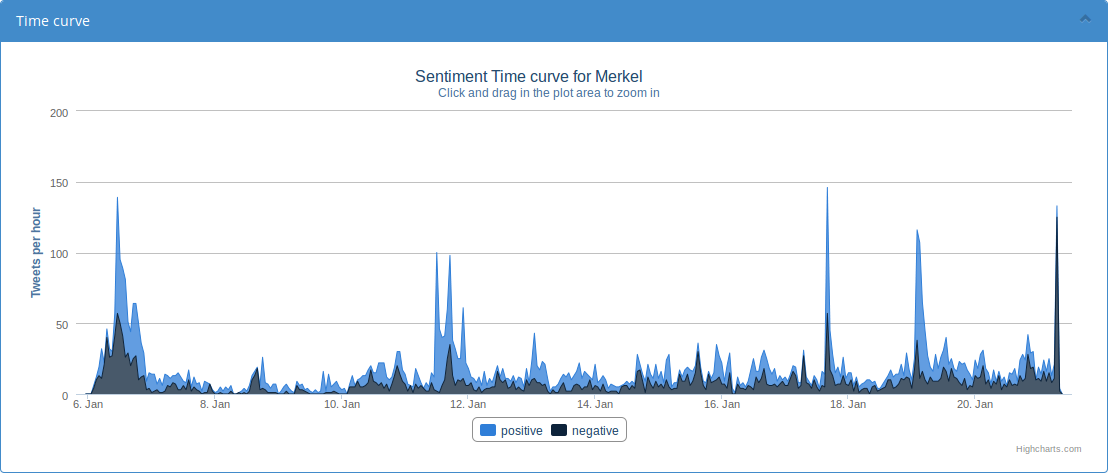
\includegraphics[width=0.8\textwidth]{Bilder/Frontend/Screenshots/sentimentPerHour-oldVersion.png}
\caption{Vorherige Version der Sentimentdarstellung im zeitlichen Verlauf.}
\label{img:SentOverTimeOld}
\end{figure} 

Daher wurde eine abweichende Darstellung entwickelt, welche das relative Verhältnis zwischen positiven und negativen Tweets darstellt. Dies ermöglicht dem Benutzer deutlich besser zu erkennen, wie sich das Meinungsbild zu dem jeweiligen Suchbegriff über den zeitlichen Verlauf entwickelt hat.

Aber auch bei dieser Darstellung gab es zwei verschiedene Probleme. Zum einen gab es unabhängig von der zeitlichen Auflösung immer einige Bereiche in denen es keine Tweets gab, weder positive noch negative, sodass viele Lücken in dem Graphen vorhanden waren, was es schwerer machte, diesen zu interpretieren. Zum anderen gab es ebenso Zeitpunkte, in denen nur positive oder nur negative Tweets gefunden werden konnten, sodass auch hierdurch die Darstellung stark zerhackt wurde. Diese Probleme wurden durch den Einsatz eines gleitenden Mittelwertes behoben. Der Graph zeigt somit zu jedem Zeitpunkt den Durchschnitt des Verhältnisses zwischen positiven und negativen Tweets der vorherigen 24 Stunden an.

\begin{figure}
 \centering
 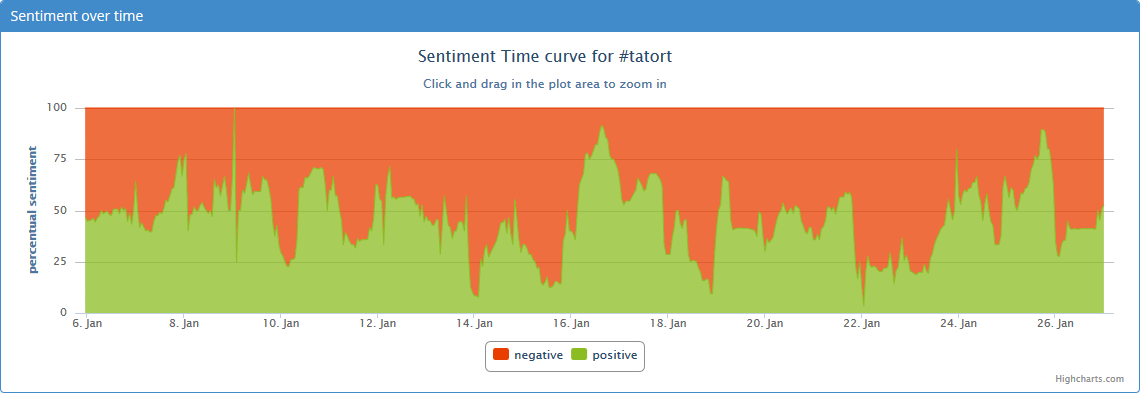
\includegraphics[width=0.8\textwidth]{Bilder/Frontend/Screenshots/latestSentimentPerHourTatort.png}
\caption{Finale Version der Sentimentdarstellung im zeitlichen Verlauf.}
\label{img:SentOverTimeFinal}
\end{figure} 

Diese Darstellung wurde von allen Beteiligten direkt verstanden und kann intuitiv auch ohne weitere Erklärungen von jedem Benutzer erfasst werden. (Siehe Abbildung \ref{img:SentOverTimeFinal}.)

\subsubsection{Performance der Tag Cloud}
Die Darstellung der Tag Cloud funktioniert wie gewünscht, es konnten jedoch Ladeprobleme bei den anderen Analysen beobachtet werden, seit die Tag Cloud zu den Auswertungen hinzugefügt wurde. Teilweise stockte die gesamte Darstellung der Auswertungen. Erste Überlegungen in Richtung Datenübertragung oder Verzögerungen auf Serverseite wurden schnell zerstreut, da andere Auswertungen hier länger auf Daten warten müssen und die Darstellung anderer Auswertungen hierdurch nicht verzögert wird.

Die weitere Analyse beschäftigte sich also mit dem Aufbau der eingesetzten Fremdkomponenten. Dies ergab, dass die \texttt{d3-cloud}-Bibliothek für jeden Eintrag einer Liste von Wörtern versucht, eine mögliche Position zu ermitteln. Diese Positionsermittlung geschieht in zentrischen Spiralen und benötigt dazu exakte Informationen über die Ausdehnung des jeweiligen Wortes, um auch die Lücken zwischen einzelnen unterschiedlich hohen Buchstaben des selben Wortes ausnutzen zu können. Versuche ergaben, dass sich unabhängig von der Länge dieser Liste die Anzahl der anzeigbaren Worte circa auf 100 belief. Obwohl der verfügbare Platz zur Anzeige ab dann nahezu vollständig aufgebraucht war, wurden genannte Berechnungen für jedes weitere Wort in der Liste vorgenommen. Diese Berechnungen konnten mittels kürzerer Listen als die Ursache für die beobachteten Probleme identifiziert werden. Obwohl mittels JavaScript-Timer- und Intervall-Funktionen versucht wurde für diese Berechnungen eine gewisse Asynchronität zu erreichen, sodass diese Berechnungen nicht mehr zwingend am Stück durchlaufen müssen, sondern von dem JavaScript-Interpreter unterbrochen werden können, um zunächst die anderen Auswertungen darzustellen, war dieser Ansatz von unzureichendem Erfolg gekrönt. Die Begrenzung der Liste schien das adäquate Mittel der Wahl zu sein, zusammen mit den Optimierungen in Punkto asychroner Ausführung konnte somit eine zufriedenstellende Performance-Optimierung erreicht werden, ohne durch eine zu große Beschränkung der Liste Nachteile im Detailgrad der Darstellung in Kauf nehmen zu müssen.

Zwischenzeitlich kam die Idee auf, die gesamte Berechnung evtl. auf den performanteren Server zu verlagern. Da die Darstellung der Tag Cloud aber von dem verfügbarem Platz auf der Webseite und vor allem auch von der verwendeten Schriftart abhängig ist, lässt sich diese Berechnung in zufriedenstellendem Maße nur im Browser bewerkstelligen.
Andernfalls hätte eine komplette Neuentwicklung der Tag Cloud stattfinden müssen, welche im Ergebnis fertige Grafiken zum Browser übertragen hätte und nicht wie es aktuell der Fall ist, lediglich eine schmale Liste von Wörtern im JSON-Format. Dieser Ansatz wurde daher auch sehr schnell wieder verworfen.

\subsubsection{Sprachfilter}
Die Idee der Einbindung eines Sprachfilters entstand, nachdem die Ansicht der Sprachverteilung implementiert war und der Kunde den Wunsch hegte, einzelne Sprachen eines Suchbegriffs genauer analysieren zu können. Der Sprachfilter ist eine globale Einstellung und wirkt sich auf die Auswertungen aller Suchbegriffe aus, die der Benutzer angezeigt bekommt.

Auf dieser Basis musste nun entschieden werden, wo in der Anzeige des Sprachfilters am besten einzubauen ist. In der ersten Version wurde ein einfaches Dropdown-Menü in der Navigationsleiste der Seite verwendet. Wie in Abbildung \ref{fig:langFilter1} zu sehen ist, war dieser Ansatz aber funktional getrieben, da die Anzeige des Sprachfilters nicht in das optische Gesamtkonzept integriert ist. Im zweiten Konzept (siehe \ref{fig:langFilter2}) fügt sich der Sprachfilter nun optisch ins Gesamtbild ein. Die Anbringung an die Suchleiste soll dem Benutzer suggerieren, dass es sich um eine Filterfunktion handelt und nicht um eine Einstellung der Anzeigesprache der Seite. Ein Problem ist allerdings, dass eine Änderung des Sprachfilters nur möglich ist, wenn die Suchleiste auch sichtbar ist. Da die Suchleiste aber verschwindet, wenn der Benutzer bei der Analyse der Ansichten nach unten scrollt, bedeutet dies, dass der Benutzer zunächst wieder nach oben scrollen muss, bevor der Sprachfilter geändert werden kann. Vor allem bei mobilen Endgeräten tritt dieses Problem aufgrund der geringeren Höhe der Ausgabe häufig auf. Aus dieser Überlegung entstand in der Folge das finale Konzept (siehe \ref{fig:langFilter3}), bei dem eine homogene Einbindung in die Navigationsleiste vorliegt. Daher ist der Sprachfilter auch immer sichtbar und verfügbar, da die Navigationsleiste beim Scrollen immer sichtbar bleibt.

\begin{figure}[ht]
\centering
\begin{subfigure}[t]{0.8\textwidth}
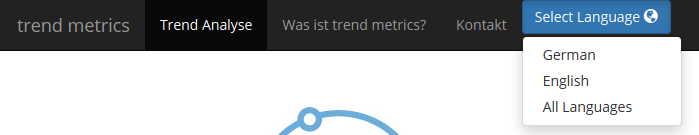
\includegraphics[width=\textwidth]{Bilder/Frontend/Screenshots/languageFilter1.png}
\caption{Erste Version des Sprachfilters. Ansatz: Funktionalität statt Design.}
\label{fig:langFilter1}
\end{subfigure}
\vspace*{5mm}
\begin{subfigure}[t]{0.8\textwidth}
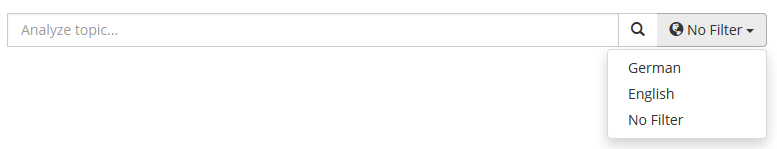
\includegraphics[width=\textwidth]{Bilder/Frontend/Screenshots/languageFilter2.png}
\caption{Zweite Version des Sprachfilters. Ansatz: Sprachfilter an der Suchleiste.}
\label{fig:langFilter2}
\end{subfigure}
\vspace*{5mm}
\begin{subfigure}[t]{0.8\textwidth}
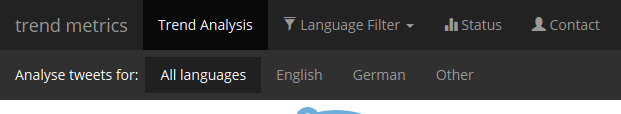
\includegraphics[width=\textwidth]{Bilder/Frontend/Screenshots/languageFilter3.png}
\caption{Finale Version des Sprachfilters. Ansatz: Integration in die Navigationsleiste}
\label{fig:langFilter3}
\end{subfigure}

\caption{Vergleich der verschiedenen Layouts des Sprachfilters}
\label{fig:langFilter}
\end{figure}

\subsubsection{Warnungen und Fehler}
Damit mögliche Fehler als Antwort einer Anfrage vom REST-Service nicht zum Absturz des gesamten Frontends führen, ist es notwendig, angemessen auf Fehler zu reagieren.
Wenn der HTTP Status Code der Antwort nicht \texttt{200 OK} lautet, handelt es sich um einen Fehler, bzw. ist ein Fehler im REST-Service aufgetreten. Eine Warnung liegt vor, wenn die Antwort vom REST-Service fehlerfrei vorliegt, aber nicht genügend Daten vorhanden sind, um vernünftige Auswertungen anzeigen zu können.

Die Anzeige der Fehler und Warnungen erfolgte zunächst in einer separaten Box, die aber nur die Anzeige eines einzigen Fehlers ermöglichte. Diese Einschränkung wurde getroffen, damit der Benutzer nicht von einer Flut an Fehlermeldungen erdrückt wird, falls die Verbindung zum REST-Service nicht fehlerfrei abläuft und somit jede Anfrage fehlschlägt.

Da aber Fehler und Warnungen immer mit einer Anfrage an den REST-Service verknüpft sind, erschien es im Laufe der Entwicklung vernünftig, dies auch optisch durch die Anzeige von Fehlern und Warnungen in den einzelnen Auswertungsboxen hervorzuheben. Fehlermeldungen, die nicht mit einer einzelnen Auswertung zusammenhängen, werden weiterhin in einer separaten Box angezeigt. Allerdings können diese Meldungen nun, ähnlich wie ein Fenster einer Anwendung in Windows, in der rechten oberen Ecke geschlossen werden, sodass der Benutzer selbst entscheiden kann, wann eine Meldung für ihn nicht mehr relevant ist.

Zusätzlich dazu wurden auch noch Fehlercodes eingeführt, die in den Fehlermeldungen angezeigt werden. Diese stellen einen Kompromiss zwischen möglichst exakter Fehlerbeschreibung für den Entwickler und Vermeidung unnötiger Details für den Benutzer dar.

\subsection{Diskussion}
Die Entwicklung des Frontend hat gezeigt, dass man diesen Teil nicht vollständig von der darunter liegenden Schicht loslösen kann und dass die Absprachen in unserem Fall mit dem REST-Service weit über eine Verständigung über die zu verwendende API hinausgehen müssen.
So muss man bei der Konzeption frühzeitig einige mögliche Problemstellen berücksichtigen, wie z.B. die auf im Schnitt maximal sechs mögliche parallele Verbindungen begrenzte Kapazität der Browser-Server-Verbindungen. Man sollte seine Anwendung also auf keinen Fall so bauen, dass man auf viele parallele Verbindungen angewiesen ist, und falls sich dies nicht vermeiden lässt, dass diese auf jeden Fall sehr schnell terminieren um weiterer Verbindungsversuche des Browsers nicht zu blockieren. Dies würde den Browser ansonsten schnell einfrieren oder der Benutzer erhält den Eindruck, dass seine Anwendung gerade hängen geblieben ist.
Diese Probleme lassen sich durch frühzeitige Konzepte wie z.B. einer Art Mulitplexing umgehen, welche hier nicht weiter ausgeführt werden sollen.

Des Weiteren haben wir erkannt, welche Berechnungen man browserseitig anstellen sollte und welche Berechnungen auf dem Server besser aufgehoben sind. Die Tag Cloud ist hier ein sehr schönes Beispiel. Aufgrund der Vielzahl unterschiedlicher Systeme, die auf einen Webservice zugreifen, kann man auf dem Server keinerlei Annahmen über die beim Besucher vorhandenen Schriftarten machen, welche browserseitig dynamisch für die Anzeige der Wörter verwendet werden. Somit lassen sich die exakten Positionen nicht auf dem Server ermitteln und diese Berechnung muss im Browser stattfinden. Dennoch sollte man sich an dieser Stelle stets der eingeschränkten Möglichkeiten von JavaScript bewusst sein, da zumindest zum heutigen Datum noch keine parallelen Ausführungen von Java\-Script möglich sind und zu umfangreiche Berechnungen den Browser sehr schnell blockieren können.
Eine sinnvolle Abwägung ist also unabdingbar.

Durch die verschiedenen optischen Ansätze des Frontends ist ebenfalls deutlich geworden, dass auch hier eine detaillierte konzeptionelle Vorarbeit notwendig ist, um spätere weiträumige Änderungen auf ein Minimum zu reduzieren. Weitreichende Änderungen bis hin zu kompletten Neuentwicklungen sind im Verlaufe eines Projektes oftmals sehr schwierig und dann nur mit einem erheblichen Mehraufwand zu bewerkstelligen. Dennoch hat der Verlauf des Projektes hier auch gezeigt, dass man selten im Voraus alle Anforderungen exakt kennt und gerade diese Komponente durch eine starke Nähe zum Kunden flexibel reagieren können muss. Frühzeitige Überlegungen gemeinsam mit dem Kunden, wie das Frontend aussehen soll und eventuell die Anfertigung eines funktionslosen Prototypen können mögliche Wege sein, unnötige Änderungen im späteren Verlauf zu vermeiden.
Dennoch kann man festhalten, dass die ändernden Anforderungen zusammen mit dem flexiblen Unterbau in Form des HTML5-Frameworks Bootstrap \cite{Bootstrap} zu einem sehr zufriedenstellenden Ergebnis geführt haben. Trotz aller Änderungen ist es uns daher gelungen, die gewünschten Anforderungen umzusetzen und sogar zu übertreffen.